\section{Method}
\label{sec:method}

The audit first measures the additional score loss from masking annotated answer evidence rather than comparable non-evidence content. It then asks whether a specified internal object reproduces the score change caused by the evidence mask. Within each internal comparison, we hold the image--question example, answer target, corruption, and readout fixed. We compare effects at specified interfaces without assuming that sparse features or internal coordinates are shared across models.

\subsection{Answer scores and matched visual damage}

For an image--question input $x$ and fixed target answer $a=(a_1,\ldots,a_T)$, a condition $c$ specifies one complete model run, including any image corruption or internal intervention. We supply the fixed prefix before each answer token so that all paired runs score the same answer. If $p_t^c$ is the model probability of target token $a_t$ under this condition, the primary complete-answer score is
\begin{equation}
S_{\mathrm{seq}}(x,a;c)=\sum_{t=1}^{T}\log p_t^c .
\label{eq:sequence-score}
\end{equation}
First-token logit and rank scores and correct-versus-wrong margins provide complementary readouts; their exact definitions are in Appendix~\ref{app:detailed-method}. Let $c_0$ be the clean run, $c_{\mathrm{evid}}$ the annotated evidence-mask run, and $c_{\mathrm{ctrl}}$ a run masking a same-area random non-evidence region. For any fixed answer score $S$, define
\begin{align}
D_S(x,a;c)&=S(x,a;c_0)-S(x,a;c), \label{eq:corruption-damage}\\
E_S(x,a;c_{\mathrm{evid}},c_{\mathrm{ctrl}})
&=D_S(x,a;c_{\mathrm{evid}})-D_S(x,a;c_{\mathrm{ctrl}}).
\label{eq:evidence-control-contrast}
\end{align}
The first quantity is the clean-to-masked answer-score loss. A positive second quantity means the annotated evidence mask causes more loss than its matched control. Figure~\ref{fig:visual-mask-example-main} illustrates these matched inputs on one question before the aggregate tests.

\begin{figure}[!htbp]
\centering
\begin{minipage}{0.31\linewidth}
\centering
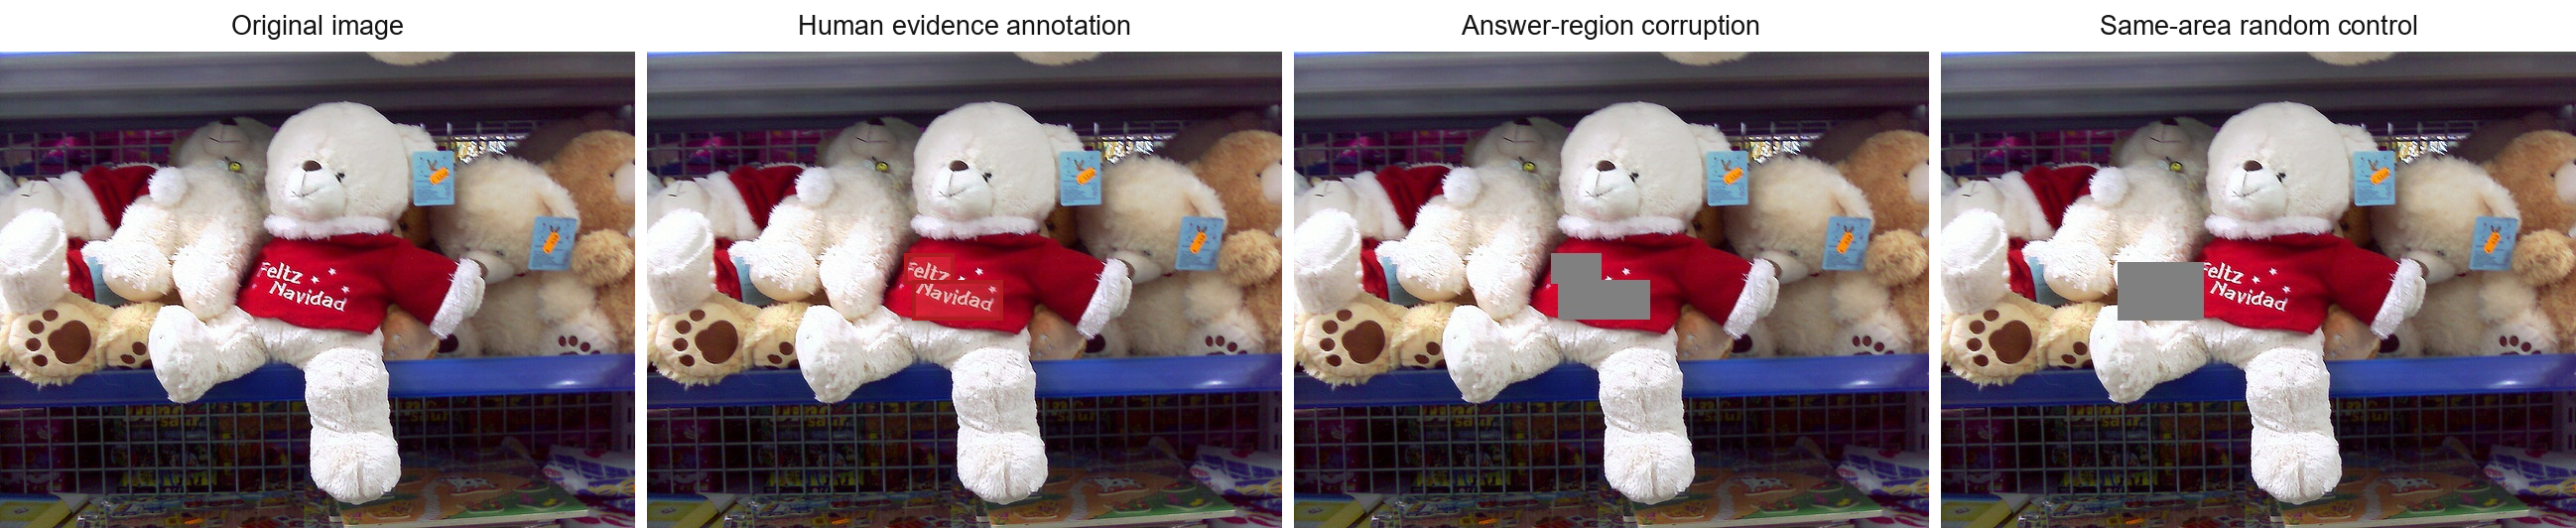
\includegraphics[width=\linewidth,trim=0bp 130bp 1947bp 90bp,clip]{figures/okvqa_val_4739195_input_control_panel.png}
\normalsize (a) Original
\end{minipage}\hfill
\begin{minipage}{0.31\linewidth}
\centering
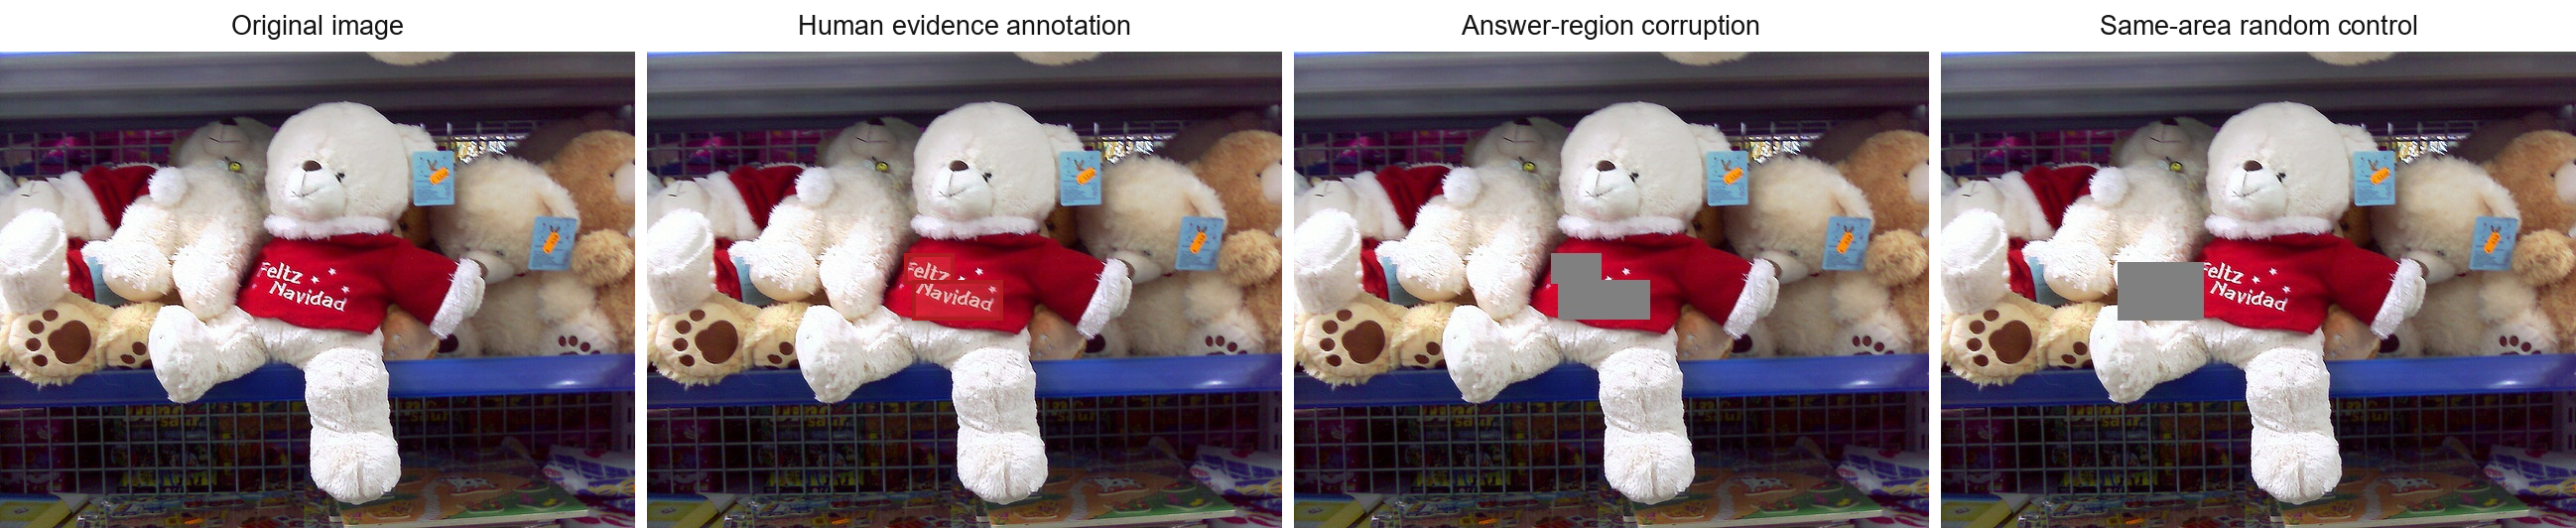
\includegraphics[width=\linewidth,trim=1298bp 130bp 649bp 90bp,clip]{figures/okvqa_val_4739195_input_control_panel.png}
\normalsize (b) Evidence masked
\end{minipage}\hfill
\begin{minipage}{0.31\linewidth}
\centering
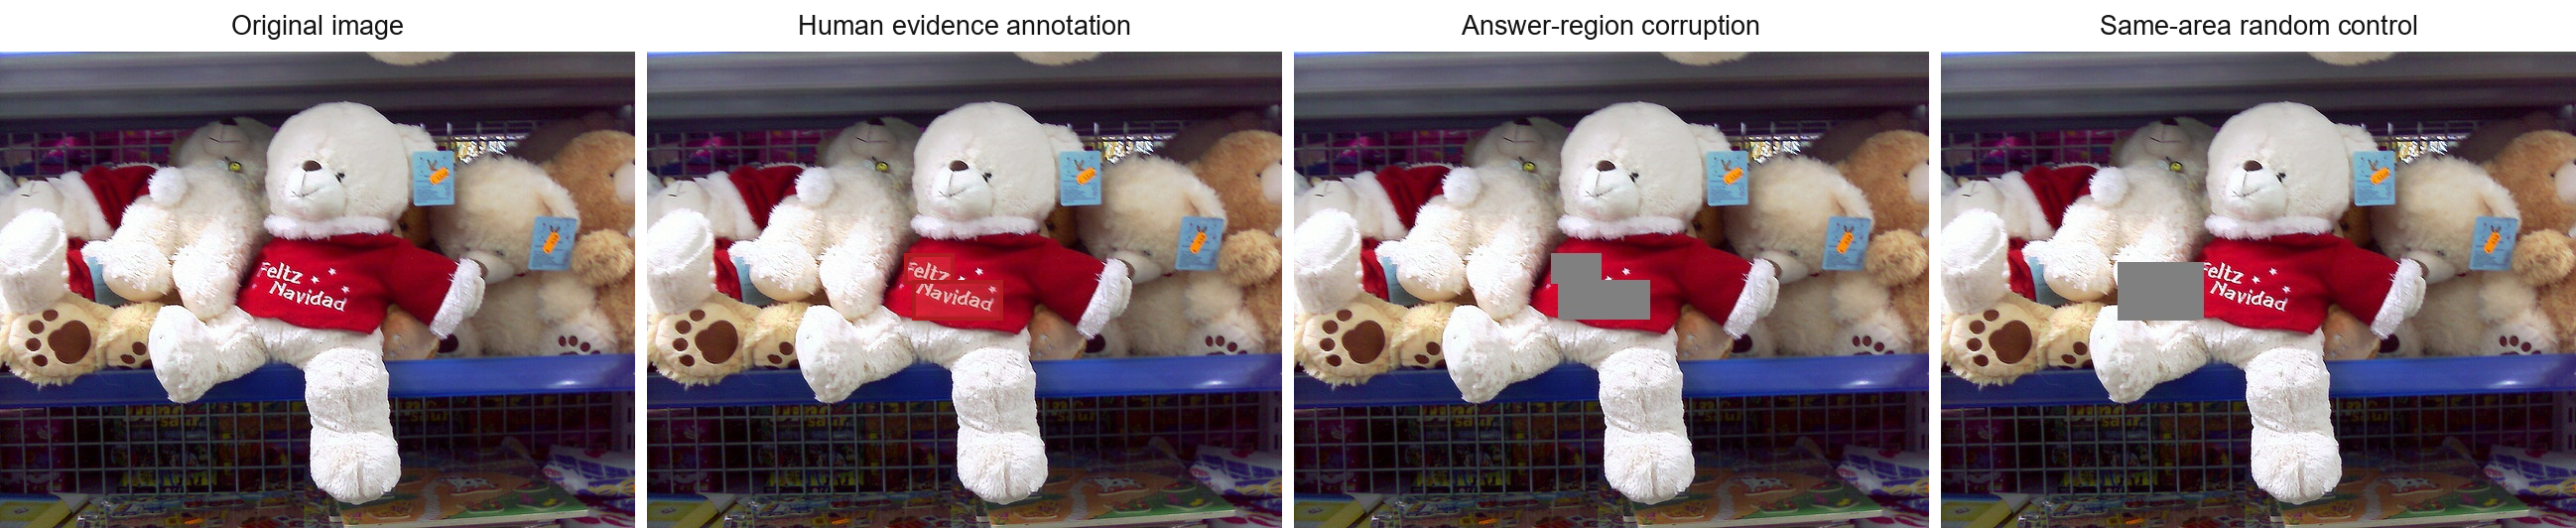
\includegraphics[width=\linewidth,trim=1947bp 130bp 0bp 90bp,clip]{figures/okvqa_val_4739195_input_control_panel.png}
\normalsize (c) Same-area control
\end{minipage}
\caption{\textbf{The matched visual comparison on one compact-evidence question.} For ``What language is the sign on the bear in?'' the target answer is ``Spanish.'' Gray corruption covers the annotated text in (b) and an equally sized non-evidence region in (c). The panels illustrate the paired input conditions, not a single-case mechanism result; the full human annotation is shown in Appendix~\ref{app:annotation-protocol}.}
\label{fig:visual-mask-example-main}
\end{figure}
\FloatBarrier

\subsection{Testing internal objects in both directions}

At a specified layer and position group, let $o$ be the complete dense state or a restricted candidate derived from it. $\mathtt{Restore}(o,c)$ writes the clean value of $o$ into a corrupted run $c$. $\mathtt{Delete}(o,c)$ is shorthand for writing the value recorded under $c$ into the otherwise clean run; it does not zero the object. Their target-score effects are
\begin{align}
B_S(x,a;o,c)&=S(x,a;\mathtt{Restore}(o,c))-S(x,a;c),
\label{eq:restoration-benefit}\\
A_S(x,a;o,c)&=S(x,a;c_0)-S(x,a;\mathtt{Delete}(o,c)).
\label{eq:deletion-damage}
\end{align}
Restoration measures recovered support; corrupted-state replacement measures support lost from the clean run. The two writes use the same paired state difference in opposite baseline runs, so they are complementary intervention tests rather than independent samples. A clean state copied into a damaged run can improve an answer without showing that the state was needed in the clean run; a masked state inserted into a clean run can lower the score without showing that the clean state would rescue a damaged input. We therefore compare both effects with the same natural clean-to-mask score loss. A large intervention effect alone is not enough: recovery far above the natural loss also fails to reproduce it faithfully.

Candidate classes include complete hidden states, a fitted sparse reconstruction and its remaining reconstruction error at the same feed-forward output, selected native feed-forward channels, and a low-rank hidden-state subspace shared across examples within one model. The sparse tool is a separate measurement interface; native channels belong to the base model. References differ: full feed-forward output for sparse reconstruction, all channels for native groups, and the natural clean-to-mask score change for shared subspaces and full hidden states. Each candidate must meet its own reference and control gates in both directions before we call it a complete path. Appendix~\ref{app:detailed-method} gives the feature selection, decoder reconstruction, residual, subspace projection, and intervention details; the next section fixes the evaluation sets and statistical criteria.
